% Standalone TikZ figure for Figure 4: Homogeneous (left) vs Heterogeneous (right) jury comparison (grayscale)
% Honest reference frame (per Section 5.3 revision): the reference for the
% "reduction" is the THEORETICAL degenerate bound (rho_eff=2.00), and the
% heterogeneous value (1.44) is NOT below the empirical temperature-perturbed
% homogeneous baseline (1.3692). No correlation-reduction claim is made.
\documentclass[tikz,border=4pt]{standalone}
\usepackage{tikz}
\usetikzlibrary{positioning,fit,arrows.meta,calc}
\tikzset{
  box/.style={rectangle,rounded corners,inner sep=6pt,align=center,font=\footnotesize,minimum width=28mm,minimum height=10mm,draw=black!70,fill=black!6},
  arrow/.style={-{Stealth[length=3mm]},thick,black!80},
  title/.style={font=\bfseries\small},
  note/.style={font=\scriptsize,align=center}
}
\begin{document}
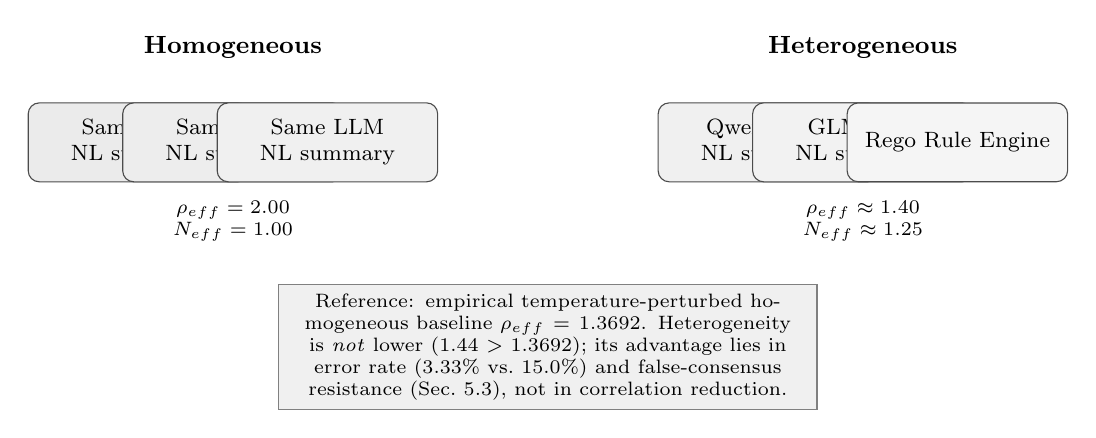
\begin{tikzpicture}
\coordinate (L) at (-4,0);
\coordinate (R) at (4,0);

% Left: Homogeneous (same model)
\node[title] (leftt) at ($(L)+(0,1.2)$) {Homogeneous};
\node[box,fill=black!8,draw=black!70] (lh1) at ($(L)+(-1.2,0)$) {Same LLM\\NL summary};
\node[box,fill=black!7,draw=black!70] (lh2) at ($(L)+(0,0)$) {Same LLM\\NL summary};
\node[box,fill=black!6,draw=black!70] (lh3) at ($(L)+(1.2,0)$) {Same LLM\\NL summary};
\node[note] (lrho) at ($(L)+(0,-1.0)$) {$\rho_{eff}=2.00$\\$N_{eff}=1.00$};

% Right: Heterogeneous (different models)
\node[title] (rightt) at ($(R)+(0,1.2)$) {Heterogeneous};
\node[box,fill=black!6,draw=black!70] (rh1) at ($(R)+(-1.2,0)$) {Qwen2.5-3B\\NL summary};
\node[box,fill=black!5,draw=black!70] (rh2) at ($(R)+(0,0)$) {GLM-4-9B\\NL summary};
\node[box,fill=black!4,draw=black!70] (rh3) at ($(R)+(1.2,0)$) {Rego Rule Engine};
\node[note] (rrho) at ($(R)+(0,-1.0)$) {$\rho_{eff}\approx1.40$\\$N_{eff}\approx1.25$};

% Honest reference-frame note (no correlation-reduction claim)
\node[note,text width=66mm,fill=black!6,draw=black!50] (mid) at (0,-2.6) {Reference: empirical temperature-perturbed homogeneous baseline $\rho_{eff}=1.3692$. Heterogeneity is \emph{not} lower (1.44 $>$ 1.3692); its advantage lies in error rate (3.33\% vs.\ 15.0\%) and false-consensus resistance (Sec.~5.3), not in correlation reduction.};

\end{tikzpicture}
\end{document}
